\documentclass[10pt]{article}
\usepackage[subtle]{savetrees}
\usepackage[hidelinks]{hyperref}
\usepackage[numbers]{natbib}
%\renewcommand*{\bibfont}{\raggedright}
\usepackage{parskip,amsmath,amssymb,booktabs,float,graphicx,geometry,url}
\geometry{
 a4paper,
 right=15mm,
 left=15mm,
 top=15mm,
 bottom=15mm
 }
\title{
    \textsc{\huge User Guide }\hfill \textsc{\small CEGE0016: Group Coursework Project 22/23 }\\%[0.3cm]
    \textsc{\large Group 7} \hfill \textsc{\small University College London }\\
    \ \hfill \textsc{\small \today }
    \vspace{-3em}
}
\date{}
\author{}
\begin{document}
\maketitle
\section{Methodology}
Play region selected: Outer perimeter of Stamford Bridge

Rationale: Largest fracking potential likened to American wells that forms basis of project estimations.
\subsection{Benefits}
\subsubsection{Economic growth from increased purchasing power}
Increased employment results in increased purchasing power locally. 35.3\% of O\&M cost accounts for wages \cite{001}. Net wages obtained by deducting 30\% income tax. The average household saving ratio is 8.34\%, thus, 91.66\% of wages are spent locally \cite{002}. Initial contribution into the economy acts as economic stimulus that is quantified using a multiplier \eqref{MPC} where MPC is 11\% \cite{003}. Multiplier $\times$ initial contribution gives yearly values of economic growth. Values accumulated and discounted by predicted inflation to obtain present values.
\begin{equation}\label{MPC}
    \frac{1}{1 - \textrm{Marginal Propensity to Consume}}
\end{equation}
\subsubsection{Tax revenue from salaries}
Wages of well-site employees are taxed \cite{004} at 30\%. The tax revenue is accumulated yearly using the same method above.
\subsubsection{Revenue from sale of shale gas}
Natural gas prices are predicted by Deloitte for years up to 2051 \cite{005}. These prices (USD) are converted at the average exchange rate for year 2022 (\$1:\pounds0.8106). The production rate per well per day was estimated at 2.6 million cubic feet \cite{006}. Daily production rate adjusted for 30 wells to obtain yearly production rate. Yearly production adheres to a hyperbolic decline function with constant, $b = 0.8426$ [5], implying that production rates drop off continually. The prices per year is multiplied with yearly production rate to obtain yearly revenue. No discount rate is applied because Deloitte prediction accounts for inflation.
\subsubsection{Community charter}
The minimum package of benefits (government requirement) involves a one-time payment of \pounds 100,000 at the exploration stage of the well-site and 1\% of revenue from sale of shale gas as yearly payment to local community \cite{007}. Payments to local council assumed to be invested into local economy as an initial economic stimulus. Multiplier applied to represent compounded economic growth. One-time payment values accumulated and discounted by inflation to obtain present values. 1\% of revenue value yearly already accounted for inflation.
\subsubsection{Increase in energy security}
The highest price in 2022 was taken, given it accounts for extreme circumstances that caused skyrocketing natural gas prices. The difference between the highest price and historical average \cite{008} used to quantify value of energy security (UK has own shale gas source). Multiplying this with the production rate, energy security quantified via savings made by locally producing over importing.
\subsubsection{Greenhouse gas emissions}
The greenhouse gas emissions of shale gas were compared to that of natural gas (conventional) and imported LNG. Shale gas extraction and use is comparable to gas from conventional sources \cite{009}. Net carbon emissions were derived from production rate. Price was ascertained for the carbon emissions using a carbon emissions pricing index \cite{018}.
\subsubsection{Water consumption}
The water consumed in the production of shale gas compared to oil is significantly lower \cite{017}. The difference in water consumption can be multiplied with local water prices sourced from United Utilities to find the cost reduction associated with the reduced consumption \cite{010,011}.
\subsection{Core costs}
Overall, the core costs were predominantly obtained from Cooper \textit{et al.} and cross referenced with Mehany \textit{et al.} \cite{COOPER2018577,MEHANY2019375}.
\begin{table}[H]
    \centering
    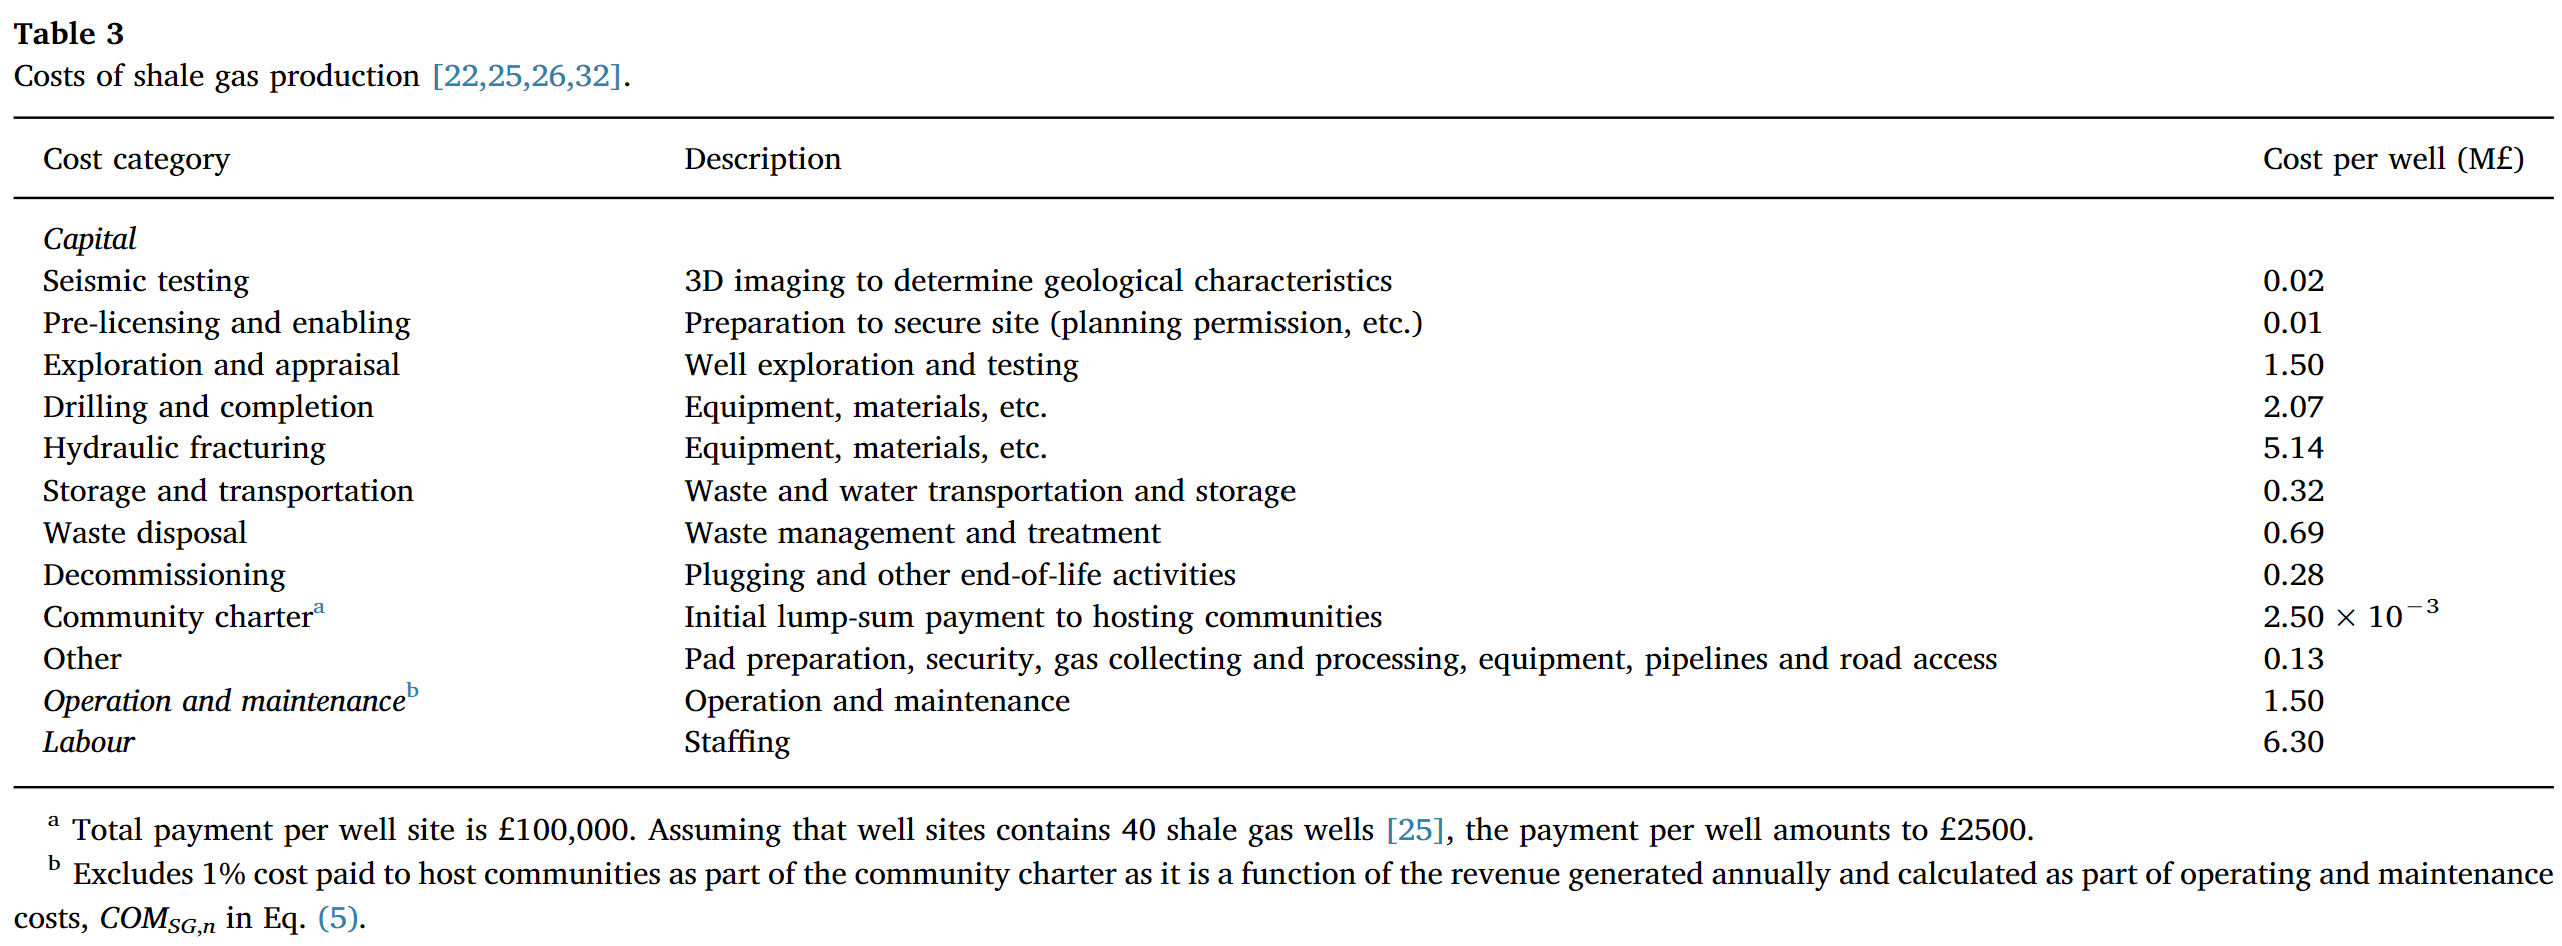
\includegraphics[width = \textwidth]{fig1.png}
    \caption{Cost per well table from reference paper \cite{COOPER2018577} (predictions for 2030).}
    \label{costsShaleGas}
\end{table}
\subsubsection{Investment costs}
\begin{itemize}
    \item Seismic testing
    \item Pre-licensing and enabling
    \item Exploration and appraisal
    \item Other
    \item Labour
    \item Community charter - initial lump sum (\pounds 100,00 per well-site)
\end{itemize}
All costs are considered up-front.``Other'' costs include large investment components i.e., pad preparation, equipment, pipelines, and road access are initial costs assumed as investment costs. Considering ``Operation and maintenance'' cost within Table \ref{costsShaleGas}, the ``Labour'' cost is assumed as an investment cost. This is the cost of contractors paid to initially set up the well sites.

\textbf{Calculation:}
Due to major macro-economic changes between the date of this paper and the current economic climate, this was adjusted to reflect a prediction for 2030 made in 2022. Therefore, the value from 2018 was adjusted for inflation (2018-2022). Finally, the estimated total cost for 2022 discounts the prediction for 2030 back to 2022 based on the predictions of inflation for the period shown in Table \ref{inflation}
\begin{table}[H]
    \centering
    \begin{tabular}{@{}ll@{}}
        \toprule
        \textbf{Inflation Rate UK Predictions} &         \\
        \midrule
        2023                                   & 7.40\%  \\
        2024                                   & 0.60\%  \\
        2025                                   & -0.80\% \\
        2026                                   & 0.20\%  \\
        2027                                   & 1.70\%  \\
        Post 2027 inflation rate               & 2.00\%  \\
        \bottomrule
    \end{tabular}
    \caption{Inflation predictions (First 5 years obtained from Statista predictions and post 2027 prediction is 2\% matching Bank of England target inflation) \cite{012}.}
    \label{inflation}
\end{table}
\subsubsection{Operation and Maintenance costs}
\begin{itemize}
    \item Drilling
    \item Hydraulic fracturing
    \item Storage and transportation
    \item Waste disposal
    \item Equipment O\&M (non-hydraulic fracturing and drilling costs i.e., electricity, labour, etc.)
    \item Community Charter - annual payments (1\% of revenue)
\end{itemize}
Costs in Table \ref{costsShaleGas} did not break down the drilling cost and completion cost. As completion is an end-of-life cost rather than a yearly cost, this makes Table \ref{costsShaleGas} values inaccurate for calculating the BCR. Therefore, drilling and well completion costs were found separately \cite{MEHANY2019375}. These were adjusted to GBP and for inflation to get a yearly cost.

After obtaining the yearly costs, the PV function was used with the payment being the yearly cost, the period being the number of years (i.e., 10, 20, 30 years depending on the workbook), and finally the MARR, estimated by the ``social discount rate'' of 3.5\%, which is commonly used for government projects \cite{013}.
\subsubsection{End of life costs}
\begin{itemize}
    \item Decommissioning
    \item Well completion
\end{itemize}
Again, decommissioning was calculated with same method as investment costs. The 2022 value was then adjusted for inflation so that it reflects the proper values for 10/20/30 years using the predictions of inflation from Table \ref{inflation}. Well completion cost was obtained using the same method as drilling. The 2022 cost was similarly adjusted for inflation accordingly.
\subsection{Externalities Costs}
The externalities costs were projected with the willingness to pay metric (WTP), a quantitative figure that highlights the maximum price a household is WTP for a certain service/product, typically obtained through surveys or estimations from historic fracking projects. The number of households within Stamford Bridge consequently drove the costing model, future projections were sourced from the ONS.
\subsubsection{Environmental}
Air and methane pollution was calculated annually across BCRs using values from other shale plays and adjusted with inflation, number of wells, etc \cite{019}. Habitat fragmentation was calculated using the WTP metric, but a specific quantitative cost could not be attached to the externality due to an absence of research. Its cost was only considered for the 10-year timespan as its effects are localised \cite{LOOMIS2017160}. The same was done for groundwater contamination, however, it was more representative due to greater information from prior projects. Contamination was considered across all time-spans due to it being an omnipresent problem \cite{019}.
\subsubsection{Social}
Traffic was calculated with the WTP metric; it was considered across all time-spans as fracking is continuous during this period \cite{doi:10.1146/annurev-resource-110320-092648}.
\subsubsection{Healthcare}
Healthcare externalities were quantified by statistical links between fracking and increased annual patients and expenditures per affliction \cite{015}. For premature birth rates, it was assumed that only households with none or one child would give birth to a premature baby. Lastly, asthma, respiratory, premature birth problems were assumed to start a year after fracking begins. Cardiac and dermatological complications were assumed to start 5 years after fracking begins \cite{016}.
\subsubsection{Economic}
Housing value decline due to fracking was calculated by considering the historical average household value decline when fracking commenced in the local area. The decline was considered a one-time occurrence for each household and was accounted for new households too \cite{doi:10.1080/21606544.2017.1398683}. The value decline was considered across the first 10 years of fracking as subsequent property values would account for fracking within the local area.
\bibliographystyle{unsrtnat}
\bibliography{refs.bib}
\end{document}